\section{Program Structure}

The application architecture follows the \textbf{Model-View-Controller (MVC)} design pattern, which was selected to ensure a clear separation of concerns between the simulation logic, the user interface, and the application flow control. This separation facilitates modular development and testing, allowing the backend logic to evolve independently of the frontend visualization.

The source code is organized into four primary packages within the \texttt{src} directory, each responsible for a distinct layer of the application:

\begin{itemize}
    \item \textbf{Model (\texttt{src.model}):} This package encapsulates the core logic of the circuit simulator. It defines the abstract base class \texttt{LogicComponent} and its concrete implementations (e.g., logic gates, adders, and memory units). The model is responsible for the state of the simulation but contains no reference to the user interface.
    \item \textbf{View (\texttt{src.view}):} This package manages the graphical user interface (GUI) using the \texttt{PySide6} framework. It includes the main application window, scene definitions (e.g., \texttt{LevelScene}, \texttt{SandboxModeScene}), and the interactive grid.
    \item \textbf{Controller (\texttt{src.control}):} The controller layer acts as the intermediary between the model and the view. It orchestrates the application lifecycle, manages the loading of levels via the \texttt{LevelFileController}, and handles user interactions by updating the model accordingly.
    \item \textbf{Infrastructure (\texttt{src.infrastructure}):} This package contains shared utilities, most notably the \texttt{EventBus}.
\end{itemize}

The high-level dependencies and relationships between these packages are illustrated in Figure \ref{fig:package_diagram}.

\begin{figure}[H]
    \centering
    \includegraphics[width=0.8\textwidth]{./assets/package_Diagramm.pdf}
    \caption{Package diagram illustrating the dependencies between the application modules.}
    \label{fig:package_diagram}
\end{figure}
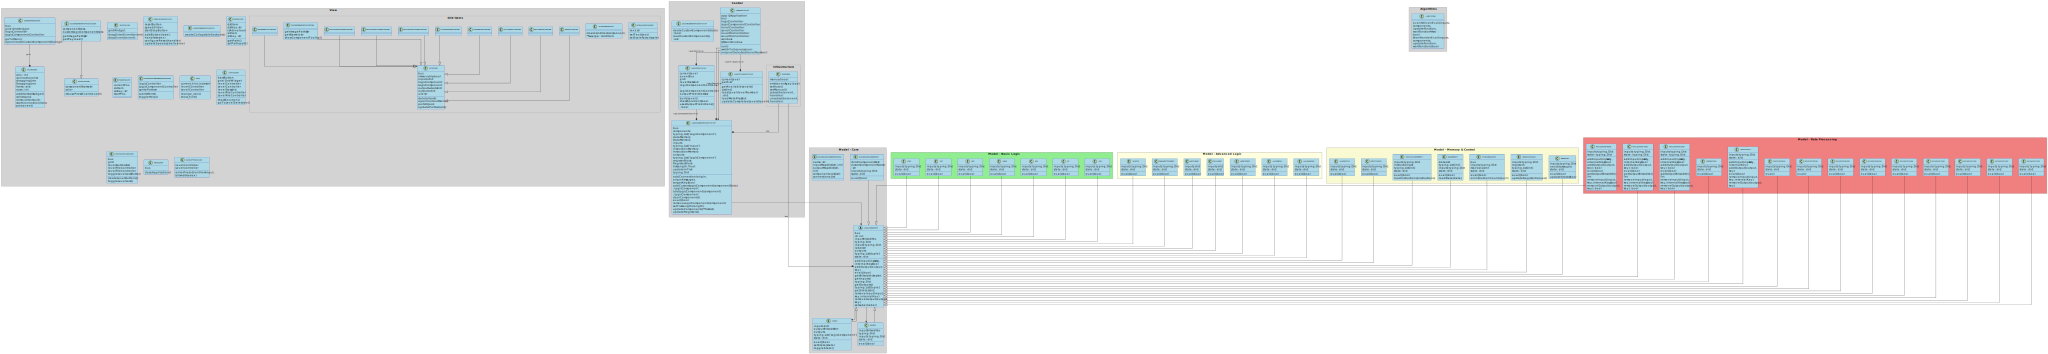
\includepdf[pages=-,fitpaper=true,angle=90]{./assets/classes_ICT-Project}
\subsection{Design Patterns and Architectural Decisions}

To maintain loose coupling between components, the project employs the \textbf{Event Bus} pattern. This is will further be explained in 6.2. Event bus and MVC decoupling.

Additionally, the \textbf{Factory Method} pattern is utilized within the view layer to manage the creation of grid items. The \texttt{GridItemFactory} class provides a static interface for instantiating the appropriate graphical representation (e.g., \texttt{InputGridItem}, \texttt{ALUAdvancedGridItem}) based on the type of \texttt{LogicComponent} provided. This abstraction isolates the \texttt{GridWidget} from the complexity of instantiating specific component subclasses, thereby adhering to the Open/Closed Principle regarding the addition of new component types.

The entry point of the application, \texttt{AppController}, initializes the main window and navigates between the distinct application states (Sandbox, Level Selection, and Level Interaction) by swapping the central widget of the main window, effectively functioning as a high-level state manager.   